\documentclass[twocolumn, a4paper, uplatex]{UECIEresume}

\usepackage{biblatex}
\addbibresource{./reference.bib}
\usepackage[dvipdfmx]{graphicx}
\usepackage{amsmath}
\usepackage{txfonts}
\usepackage{array}
\usepackage{url}
\usepackage[utf8]{inputenc}
\usepackage{booktabs}
\usepackage{nidanfloat}
\usepackage{afterpage}
\usepackage{setspace}
\usepackage{multirow}
\usepackage{here}

\usepackage{amsmath,amssymb}
\usepackage{bm}
\usepackage{subcaption}
\usepackage{verbatim}
\usepackage{wrapfig}
\usepackage{ascmac}

\usepackage{algorithm}
\usepackage{algorithmic}

\title{自然言語処理によるフェイクニュース判断の自動化}
\date{平成 31 年 2 月 15 日}
\affiliation{総合情報学科 メディア情報学 コース}
\supervisor{田原 康之 准教授}
\studentid{1510151}
\author{栁 裕太}
%\headtitle{平成 30 年度 総合情報学科 卒業論文中間発表}
\headtitle{平成 30 年度 総合情報学科 卒業論文発表}
%\headtitle{平成 yy 年度 総合情報学科 修士論文中間発表}
%\headtitle{平成 yy 年度 総合情報学科 修士論文発表}

\begin{document}
\maketitle
% 背景[フェイクニュースの自動判別の必要性+ジョークニュースを区別する必要性]+想定環境の説明(導入との被りに注意)
\section{序論}\label{ch:introduction}
%
% フェイクニュース
昨今のSNSの普及により,誰もが情報を発信・収集できるようになった.
特に最近ではテキストのみならず,画像や動画と併せて情報の発信が可能である.
一般論として,テキスト単体と比べて画像や動画と併せて発信されたマルチメディア情報の方が多くの注目を得やすい.
逆にこれを利用して,故意に情報を捏造して発信することによって人々を誤った方向へ扇動するフェイクニュースも存在する.
フェイクニュースが広まると、大規模なマイナスの影響が出る可能性があり、
場合によっては重要な公共の出来事に影響を及ぼしたり、操作したりすることさえある.
例えば2016年の米国大統領選では,2名の候補者を支持させるためのフェイクニュースが多く拡散され,
とりわけFacebook上では3700万回以上共有された\cite{10.1257/jep.31.2.211}.

% ジョークニュース
虚偽の情報ながら,扇動ではなく皮肉や風刺を込めたジョークニュースも存在する.
有名な発信メディアとしては,英語ではthe Onion,日本語では虚構新聞が該当する.
あくまで扇動ではなく笑いを提供するためのものであり,
多くの場合それは批判の的にはなりにくかった.
しかしながら,ジョークニュースはフェイクニュースと同じく限りなく真実を模した形式をとるため,
昨今では同じくSNS上で拡散されやすく,同時に批判に晒されることもある.

% 想定環境
当研究では,扇動のために故意に情報を捏造して発信された情報をフェイクニュース,
事実を発信した情報を正しいニュース,
そして風刺や皮肉を込めて発信された情報をジョークニュースとして定義する.

% フェイクニュースのテキストによる分類
フェイクニュースに限らず,風評やwebページの信憑性を評価するモデルの構築の研究は数多く行われており,
特に機械学習による分類が非常に盛んに行われている.
なかでもGranikらの研究\cite{Granik8100379}やGildaの研究\cite{Gilda8305411},そして松尾の研究\cite{松尾省吾2018master}により,
単語埋め込みとナイーブベイズ分類器やSVM,決定木といった教師あり学習を組み合わせることによって,
フェイクニュースや流言を分類するタスクで優秀な分類成果を挙げることが報告された.
ほかにもWuらの研究\cite{Wu:2018:TFF:3159652.3159677}によると,SNS上で拡散された情報に対して,
``誰が・どのような経緯で拡散したか''という情報から信憑性を判断するモデルも提案された. 
Rubinらの研究\cite{W16-0802}によれば,正しいニュース・ジョークニュースの分類にも機械学習によるアプローチが有効であることが示されていた.
正しいニュース・フェイクニュース・ジョークニュースの3カテゴリ分類においても研究が行われている.
特にHorneとSibelの研究\cite{DBLP:journals/corr/HorneA17}によると,フェイクニュースは正しいニュースよりジョークニュースに近い性質をもち,
真実に近い形式をとるほど高い説得力をもつことが示されていた.

% マルチメディアでフェイクニュース分類
上記の機械学習を使った研究では,いずれもテキストのみの情報を対象としていた.
別の対象として,テキスト・画像を併せた情報を分類する機械学習モデルの検討も数多く行われている.
大まかな形としては,まずテキスト・画像を何らかの方法でベクトル化する.
その後2種のベクトルを結合し,真偽判定を行うモデルに渡す形をとっている.
例えばJinらの研究\cite{Jin:2017:MFR:3123266.3123454}では,テキストではLSTM,画像ではVGG19を使用してベクトル化しており,
それに加えてAttentionとソーシャルコンテキスト(ハッシュタグ,URL等)により更に高精度な分類を行うモデルが提案されていた.
またWangらの研究\cite{Wang:2018:EEA:3219819.3219903}では,EANNというモデルが提案されている.
これは画像のベクトル化においては同じくVGG19を使用しているが,テキストではテキストCNNを使用していた.

上記のEANNモデルのような画像・テキスト双方を扱うモデルでは,実際に真実・フェイクとのカテゴリ分類において画像単独・テキスト単独の分類に比べて優秀な成績を収めていた\cite{Wang:2018:EEA:3219819.3219903}.\@
しかしながら,あくまで``真実なのかそうでないのか''という2カテゴリで分類しているため,
``他者を欺くための情報なのか,皮肉・風刺を込めた情報なのか''という観点での分析がなされていない.

% 本研究
本研究では,画像つきで発信された情報に対して,正しい情報か・フェイクニュースか・ジョークニュースかを判断するモデルを構築する.
このモデルを使い,従来から画像・テキスト複合のデータセットに対して3カテゴリでも優秀な分類が行えることを示すことを目指す.
それにより,SNSユーザの情報収集を支援するエージェントの開発につなげることが可能となる.

% 実験
上記の提案する情報分類システムを検証するために,
事前に用意されたデータセットを用いて10 分割交差検定によって分析を行った.
また上記システムの分類性能を評価するために,
画像・テキスト単独で分類を行った結果と比較することで,
提案システムが目標に適していることを示すことを目指した.
その結果テキスト単独でのマクロF値が約0.30,画像単独でのマクロF値が約0.47であったのに比べ,
提案モデルのマクロF値は約0.93という数値を出し,提案モデルの有効性が示された.

%全体の流れ
本論文の構成は次の通りである.
第\ref{ch:related}章では,本研究と関連のある研究や取り組みを紹介する.
第\ref{ch:purpose}章では,本研究の目的と対象とする投稿を例とともに示す.
第\ref{ch:methodology}章では,本研究が提案する手法を理論式と図とともに説明する.
第\ref{ch:experiment}章では,本研究の性能を試すために実際に評価実験を行ったため,
その詳細を記述する.
第\ref{ch:evaluate}章では,第\ref{ch:experiment}章で行った実験の結果を詳細に評価している.
考察とともに,手法や結果から浮かび上がった課題についても指摘する.
第\ref{ch:conclusion}章では,本論文をまとめるとともに,
今後の発展形についていくつかの展開を記載している.
\section{関連研究}\label{ch:related}
% フェイクニュースのテキストによる分類
正しいニュース・フェイクニュース・ジョークニュースの3カテゴリ分類を機械学習で行う研究がある\cite{DBLP:journals/corr/HorneA17}.
別の対象として,テキスト・画像を併せた情報を分類する機械学習モデルの検討も数多く行われている\cite{Wang:2018:EEA:3219819.3219903}.
画像・テキスト双方を扱うモデルでは,
実際に真実・フェイクとのカテゴリ分類において画像単独・テキスト単独の分類に比べて優秀な成績を収めていた
\cite{Wang:2018:EEA:3219819.3219903}.
しかしながら,あくまで``真実なのかそうでないのか''という2カテゴリで分類しているため,
``他者を欺くための情報なのか,皮肉・風刺を込めた情報なのか''という観点での分析がなされていない.
今回対象とする情報は,SNS上で投稿された画像つきで発信されたニュースである.
そのなかでも,正しいニュースを発信していたもの,フェイクニュースを発信していたもの,ジョークニュースを発信していたものが対象となる.

%
\section{提案手法}\label{ch:methodology}
%
\subsection{モデル概観}
この章では,提案モデルがもつ複合特徴量抽出器とニュース分類器について紹介する.
その後にこの2要素を統合して転移学習が可能な表現を学習する方法について説明する.
% 最後に,詳細なアルゴリズムフローを付加する. 
今回提案したモデルは,以下の図\ref{fig:model}の通りである.

提案モデルの目的は,画像と文章で発信された情報に対して,
正しいニュースか・フェイクニュースか・ジョークニュースかを分類するために,
必要な特徴表現を学習することであった.
提案モデルは複合特徴量抽出器とニュース分類器の大きく2部分に分けることができた.
まず複合特徴量抽出器は,今回扱う情報が文章と画像を含むため,
各メディアに対して特徴化する抽出器があった.
その後それぞれの特徴を1つに連結し,複合特徴を形成した.
複合特徴はニュース分類器に送られ,最終的には3カテゴリのどれに該当するかが判断された.
% 
\begin{figure}[H]
    \centering
    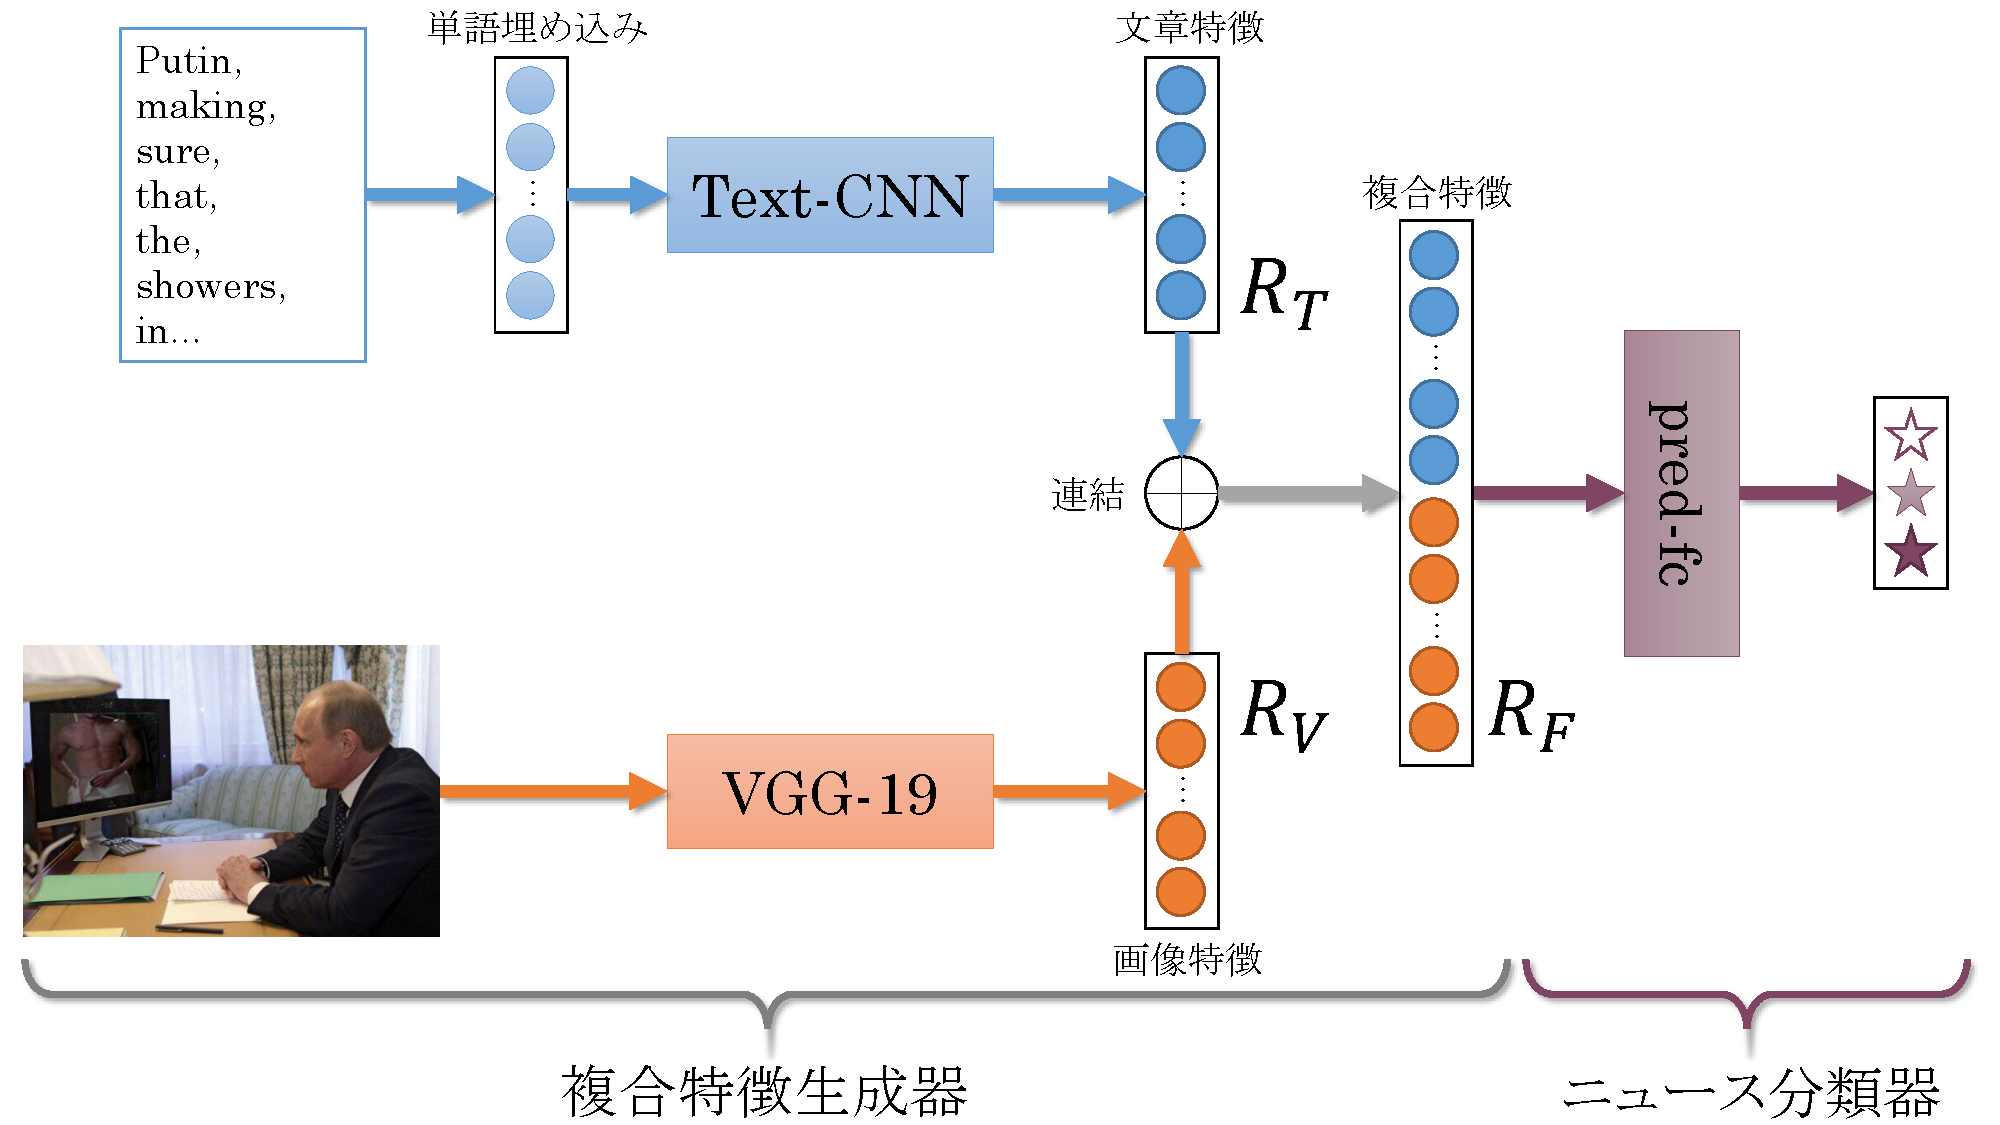
\includegraphics[width=\linewidth]{images/methodology.pdf}
    \caption{提案モデル図.青: 文章特徴量抽出器,橙: 画像特徴抽出器,紫: ニュース分類器.}
    \label{fig:model}
\end{figure}
%
\subsection{複合特徴抽出器}
%
\subsubsection{文章特徴} \label{subsec:text}
文章特徴は,入力に英語の投稿をスペース毎に分割した英単語の連続リストをもった.
まずは単語を単語埋め込みでベクトル化した.
その後単語の羅列から分類に有効な情報を得るために,文章特徴を抽出する核としてCNN
(convolutional neural networks: 畳み込みニューラルネットワーク)を採用した.
CNNはコンピュータビジョンやテキスト分類などの多くの分野で効果的であることが示されていた
\cite{collobert2011natural,KalchbrennerACL2014}.
図\ref{fig:model}の通り,提案手法ではCNNの発展形であるテキストCNN(Text-CNN)\cite{DBLP:journals/corr/Kim14f}を採用した.
テキストCNNの構造は図\ref{fig:text-cnn}の通りである.
複数のウィンドウで畳み込むことで,様々な角度から特徴を抽出することを実現した.
\begin{figure}[H]
    \centering
    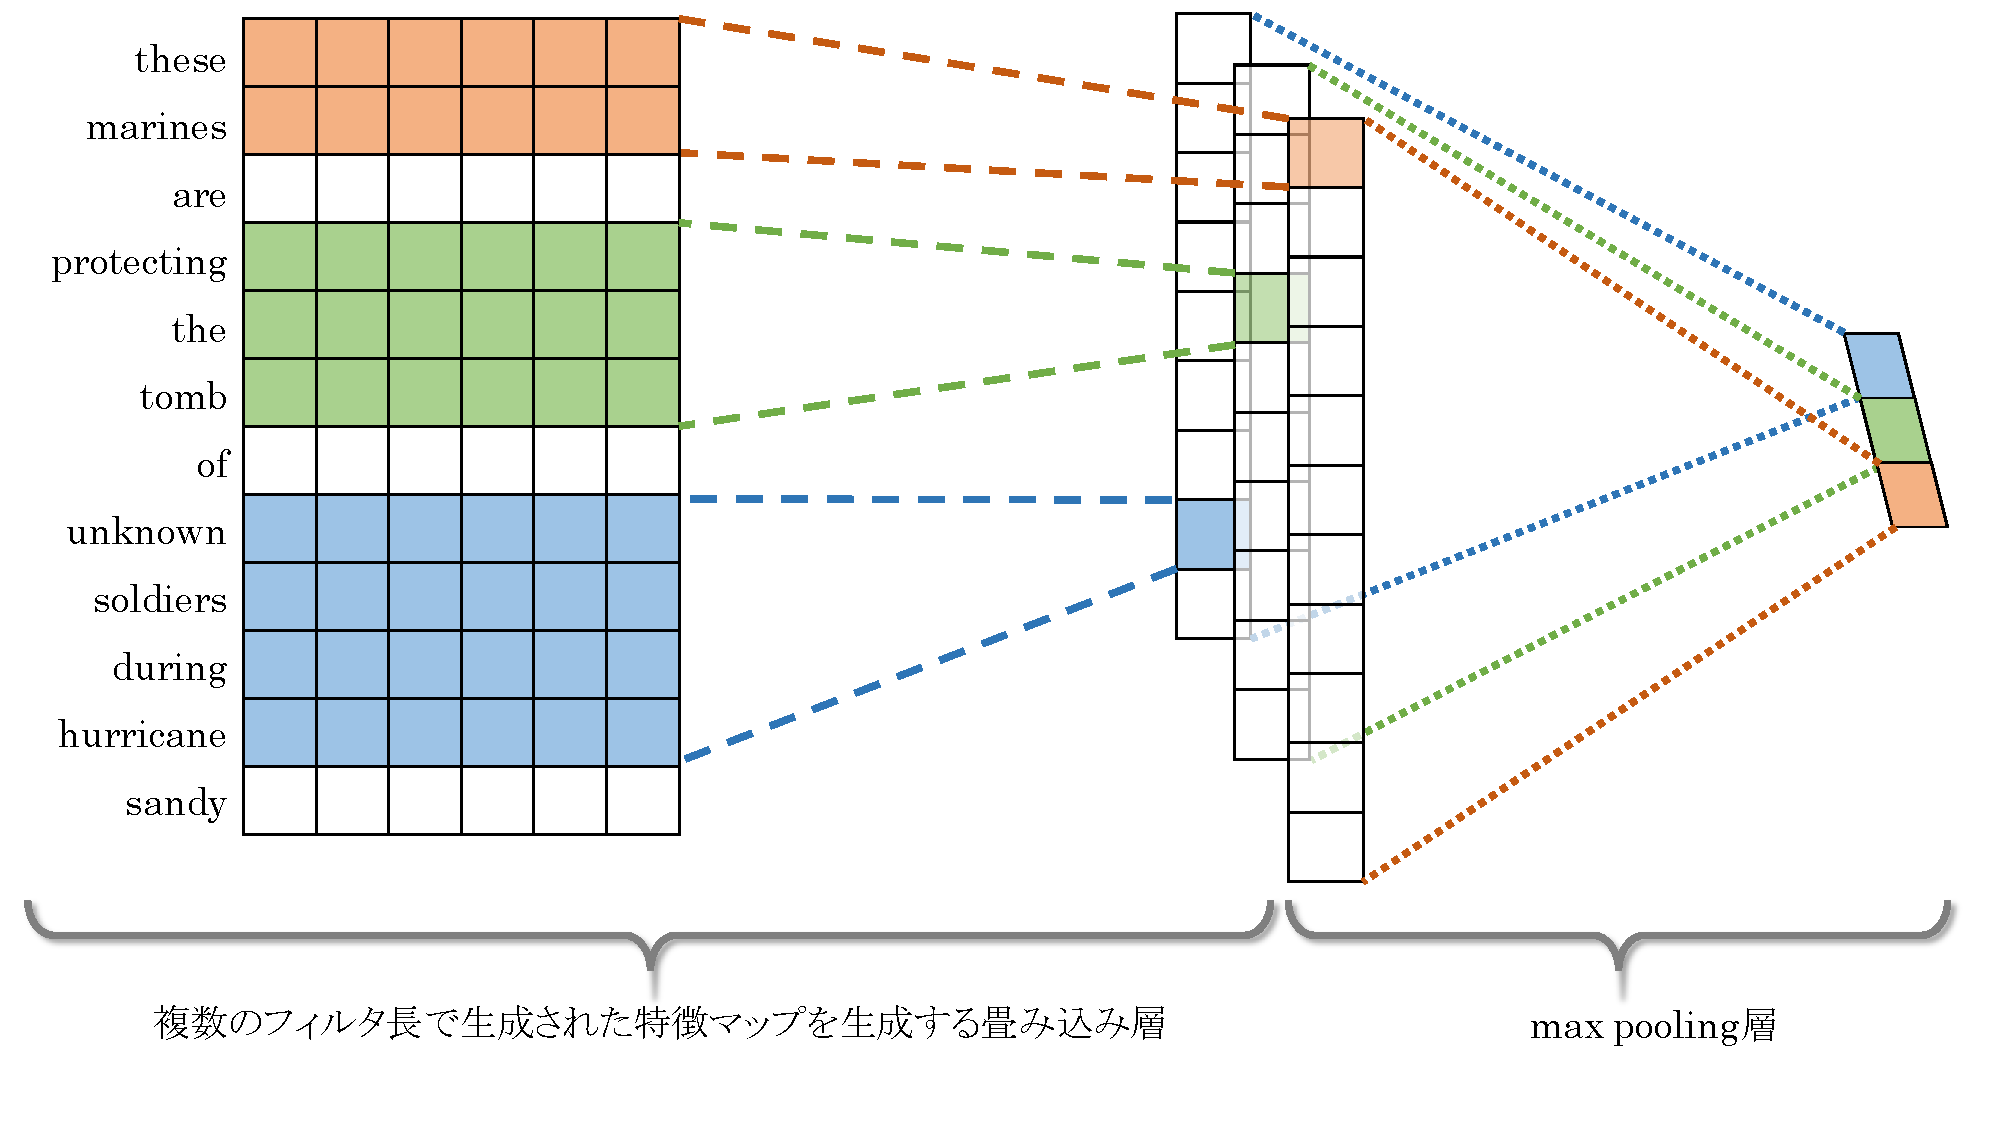
\includegraphics[width=\linewidth]{images/text-cnn.pdf}
    \caption{テキストCNNの図.Wangらの研究\cite{Wang:2018:EEA:3219819.3219903}を参考に作成.}
    \label{fig:text-cnn}
\end{figure}

具体的な手法では,EANNが採用したテキストCNNと同じ流れを汲み\cite{Wang:2018:EEA:3219819.3219903},
最終の全結合層の隠れ層に独自にdropoutを採用した形をとった.
今回使用した文章特徴抽出器の理論式を以下に引用する.

投稿の$i$番目の単語を$k$次元の単語埋め込みに変換する際に抽出された単語埋め込みベクトルを$T_i \in \mathbb{R}^k$とする.
このとき,$n$単語から抽出された投稿は以下の式\ref{eq:concat_emb}で表現ができる.
\begin{equation}
    \label{eq:concat_emb}
    T_{1:n} = T_1 \oplus T_2 \oplus \ldots \oplus T_n,
\end{equation}
$\oplus$はベクトルを連結(concatenation)することを意味する記号である.
ここで単語埋め込み化された投稿は,畳み込み層へ送られる.
畳み込み層では$h$単語分のウィンドウサイズがある.
これは単語埋め込み化された投稿から連続して取り出す単語埋め込みベクトルの数を意味する.
$i$番目を基準に$h$単語分取り出された場合,フィルタ時の処理は以下の式\ref{eq:filter}の通りである.
\begin{equation}
    \label{eq:filter}
    t_i = \sigma(W_c \cdot T_{i:i+h-1}).
\end{equation}
この$\sigma(\cdot)$は活性化関数の1つであるReLU(ランプ関数)を表し,$W_c$はフィルタの重みを意味する.
式\ref{eq:filter}が投稿内で適用されると,式\ref{eq:feature}の通り1つの発言に対し1つの特徴ベクトルが得られる.
\begin{equation}
    \label{eq:feature}
    t = [t_1, t_2, \ldots, t_{n-h+1}].
\end{equation}
この$t$ベクトルに対して最も重要な特徴を得るために,ベクトル内で最大値の要素のみを取り出すmax-poolingが行われる.

これで1つのウィンドウサイズから1つの特徴が得られるが,
多くの粒度の特徴を得るために当手法では複数のウィンドウサイズから複数の値を取得している.
特定のウィンドウサイズに着目すると,$n_h$分異なるフィルタが存在することになる.
もし使用可能なウィンドウサイズが$c$存在する場合,全体で$c \cdot n_h$だけフィルタが存在することとなる.
投稿から各ウィンドウサイズでmax-poolingまでされた文章特徴は$R_{T_c} \in \mathbb{R}^{c \cdot n_h}$と表現できる.

max-poolingを終えた文章特徴は全結合層に渡され,
最終的に式\ref{eq:image-fc}によって
画像特徴抽出器が出力する特徴ベクトルの次元($p$とする)に合わせたテキスト特徴$R_T \in \mathbb{R}^p$となる.
\begin{equation}
    \label{eq:image-fc}
    R_T = \sigma(W_{tf} \cdot R_{t_c}),
\end{equation}
ここで$W_{tf}$は全結合層における重みを意味する.なお,この全結合層では隠れ層にdropoutを当研究では採用した.
dropoutはHintonらによって提案された手法\cite{JMLR:v15:srivastava14a}で,
学習時に指定された確率で無作為に$W_{tf}$内の要素を無効化(0に)してモデルの自由度を制限することで,
モデルが訓練データセットに特化しすぎて汎用性が失われる過学習に繋がりにくくなる利点が報告されたものである.
%
\subsubsection{画像特徴}
画像から効率的に特徴を抽出するために,当研究では事前学習済みのVGG19\cite{DBLP:journals/corr/SimonyanZ14a}を起用した.
VGG19は畳み込み16層と全結合層3層から形成され,最終的には1000次元の特徴ベクトルが出力される.
当研究では最終の全結合層のみ改変し,文章特徴のベクトル次元数と同じ数の次元をもつベクトルを出力するようにした.
また改変した最終全結合層以外は,過学習を防ぐために事前学習の状態を維持することにした.
以下に,一部を改変したVGG19を利用したモデルの理論式を記す.
第\ref{subsec:text}節で記したように,最終的な特徴ベクトルの次元数は$p$とする.
VGG19では畳み込み16層で$7 \times 7 \times 512$の行列となり,
その後2層の全結合層によって$1 \times 1 \times 4096$に整形され,
最終第三全結合層(fc19)によって$1 \times 1 \times 1000$の画像特徴ベクトルを出力する.
Wangらの研究\cite{Wang:2018:EEA:3219819.3219903}ではVGGのfc19の出力を$p$に整形していたが,
当研究では直接fc19を改変して$1 \times 1 \times p$の画像特徴ベクトルを出力するようにした.
この改変したfc19によって算出される画像特徴$R_V \in \mathbb{R}^p$は以下の式\ref{eq:fc19}の通りである.
\begin{equation}
    \label{eq:fc19}
    R_V = \sigma(W_{vf} \cdot R_{V_{\rm VGGfc18}}),
\end{equation}
$R_{V_{\rm VGGfc18}}$はVGG19の第18層である全結合層が出力した$1 \times 1 \times 4096$ベクトルである.

こうして文章特徴・画像特徴が抽出され,最終的には2つの特徴ベクトルを1つに連結したものが複合特徴である.
理論式で表記すると,文章特徴$R_T$と画像特徴$R_V$が1つに結合されるため,
複合特徴$R_F$は以下の式\ref{eq:concat_feature}によって表現できる.
\begin{equation}
    \label{eq:concat_feature}
    R_F = R_T \oplus R_V \in \mathbb{R}^{2p}.
\end{equation}
以降においては,複合特徴抽出器全体を表現するときは$G_f(M; \theta_f)$と表現することにする.
$M$は複合特徴抽出器へ入力される投稿,$\theta_f$は学習対象となるパラメータを意味する.
%
\subsection{ニュース分類器}
%
複合特徴はニュース分類器(図\ref{fig:model}内`pred-fc'が該当)にて正しいニュース・フェイクニュース・ジョークニュースとして分類された.
具体的には隠れ層を含む全結合層とsoftmaxから形成され,最終的な分類が行われた.
この部分の理論式は以下の通りである.
入力となる複合特徴は$R_F$であるとき,ニュース分類器は$G_f(\cdot; \theta_d)$と表現することにする.
ここで$\theta_d$はニュース分類器内で学習対象となるパラメータを示す.
投稿全体に対して$i$番目の投稿を$m_i$とするとき,
$m_i$がフェイクニュースもしくはジョークニュースである確率は以下の式によって算出される.
\begin{equation}
    \label{eq:news_classify}
    P_\theta(m_i) = G_d(G_f(M; \theta_f); \theta_d).
\end{equation}
モデルの目的は自動で正確に正しいニュース・フェイクニュース・ジョークニュースを分類することである.
そのため正解ラベルとして$Y_d$を使用して,以下の式によってクロスエントロピー誤差を損失として算出する.
\begin{equation}
    \label{eq:cross_entropy}
    L_d(\theta_f, \theta_d) = -\mathbb{E}_{(m,y)\sim(M, Y_{d})}\biggl[\sum_{k=0}^{2} {y_k\log{P_\theta(m)}}\biggr].
\end{equation}
最後に,当研究がベースとしたWangらの研究では確率的勾配降下法(SGD: Stochastic Gradient Descent)
によってパラメータを更新していたが,
当研究では2015年にDiederik P. Kingmaらが提唱したAdamという手法\cite{DBLP:journals/corr/KingmaB14}
を用いてパラメータを更新することにした.
%


%
\section{評価実験}\label{ch:experiment}
%
\subsection{実験条件}
今実験ではTwitterデータセットを使用した\cite{boididou2015verifying}.
% 

画像つき文章投稿を3カテゴリに分類する提案手法の有効性を調べるために
文章のみで投稿を分類する手法(以降,Textと表記),もう1つは画像のみで投稿を分類する手法(以降,Imageと表記)を用意した.
いずれも上記提案モデルから文章・画像特徴抽出器を除外したモデルを使用した.
Textは入力データを提案モデルが使用したデータセットから画像を削除したものを使用し,
Imageは全投稿で使用された画像を対象とし,同じ画像に対して複数の文章投稿があった場合は1件として数えることにした.
上記の条件を踏まえ,提案手法・Text・Imageが扱う3カテゴリの投稿件数は以下の表\ref{table:posts}の通りである.

\begin{table}[h]
    \caption{提案手法と比較対象手法が扱うカテゴリ毎の投稿数}
    \label{table:posts}
    \centering
    \begin{tabular}{clll}
        \hline
        手法 & Real & Fake & Humor \\
        \hline \hline
        Text & 3021 & 4233 & 1509 \\
        Image & 172 & 157 & 82 \\
        提案手法 & 3021 & 4233 & 1509 \\
        \hline
    \end{tabular}
\end{table}

\subsection{実験結果}
3モデルに対して10分割交差検定を行った結果が以下の表\ref{table:result}の通りである.
評価指標では,Precision(精度), Recall(再現率), F値(左2値の調和平均)のマクロ平均を使用することにした.
% 
\begin{table}[h]
    \caption{各モデルの分類成果(マクロ平均)}
    \label{table:result}
    \centering
    \begin{tabular}{clll}
        \hline
        手法 & Precision & Recall & F値 \\
        \hline \hline
        Text & 0.3649 & 0.3677 & 0.3016 \\
        Image & 0.4942 & 0.5055 & 0.4667 \\
        提案手法 & 0.9268 & 0.9362 & 0.9286 \\
        \hline
    \end{tabular}
\end{table}

この結果を見ると,提案手法が他2手法と比べて非常に高い分類成果を挙げたことが読み取れた.

\section{評価}\label{ch:evaluate}

\subsection{考察}
今回の評価実験では,提案手法が3指標全てにおいて比較対象手法より優れた分類成績を収めた.
これにより,SNS上で画像つきの投稿を対象にした場合,正しいニュース・フェイクニュースの分類タスクのみならず,
ジョークニュースも含めた分類においても従来のマルチメディアモデルのアプローチが有効であることが示唆されたのではないかと考えられる.

また比較対象手法に限って結果を観察すると,文章単体より画像単体の分類の方が優秀な分類成績であった.
これは自然言語より画像の方が分類タスクにおいて研究が進んでいることや,
SNS上の投稿であった故に単語埋め込みに変換する際に\texttt{<unknown>}に変換されやすい傾向にあったことや,
文章の場合英語以外の投稿に対応できないものの,画像においては英語圏以外の投稿であっても十分言語の違いに影響されにくかったことなど,
いくつかの原因が推察される.

\subsection{課題}
今回分類するにあたり,大きな課題となったのが文章投稿の単語埋め込みへの変換であった.
例えば今回使用したデータセットがTwitterから収集されたものであったため,
事前学習済みword2vecモデルが対応できない短縮語や造語(ハッシュタグなど)といったユーザ生成コンテンツに対応することが難しかった.

また,このモデルに限らずフェイクニュース検出というタスクにおいては,Wangらの研究\cite{Wang:2018:EEA:3219819.3219903}によってある問題点が指摘されていた.
訓練に使ったデータセットが扱うイベントや出来事の特殊性の影響を受けることにより,
検証する時に訓練になかった別のイベントや出来事が使われた場合に正常な判断ができなくなる点であった.

さらに,このモデルは英語のみを対象としたものであった点も挙げられた.
データセット内一部では他国の言語が含まれていたため,単語埋め込みに変換する際に大幅に\texttt{<unknown>}に変換される傾向もあった.
%
%
\section{おわりに}\label{ch:conclusion}
%
\subsection{本論文のまとめ}
本研究では,SNS上で画像と文章を併せて発信された情報に対して,正しいニュース・フェイクニュース・ジョークニュースを判断するモデルを提案した.
実際に3カテゴリ分類を行った結果,文章・画像単体から分類した場合に比べて,全ての評価指標において非常に優秀な分類成績を挙げた.
これによりSNS上における画像つき投稿に対して,ジョークニュースを含めた3カテゴリ分類も有効であることが示された.
%
\subsection{今後の展望}
このモデルの発展として,いくつかの方法が考えられる.

データセットが扱う出来事やイベントによる特殊性の対策として,
Wangらの研究\cite{Wang:2018:EEA:3219819.3219903}では敵対的生成ネットワーク(GAN)を模倣する形をとることが挙げられていた.
真偽分類に加えて扱われたイベントも分類することによって,
フェイクニュースの普遍的な特徴を抽出するようなアプローチが行われていた.

提案手法を日本語投稿に対応させることを考えた場合,
残念ながら国内に今回使用したデータセットに近い規模をもつものがないため,
SNS上で日本語による画像つきの3カテゴリの投稿を収集する必要がある.
% 

\printbibliography[title=参考文献]
\end{document}